\chapter{GRAPHPLAN}
\thispagestyle{chapterBeginStyle}

\section{Wprowadzenie}
    \textbf{GRAPHPLAN} jest algorytmem do planowania akcji działający w dziedzinie zdefiniowanej
    przez język STRIPS, dodatkowo bazuje na paradygmacie, który autorzy algorytmu określają jako "graf planujący" \cite{GRAPHPLAN}.
    \begin{figure}[H]
        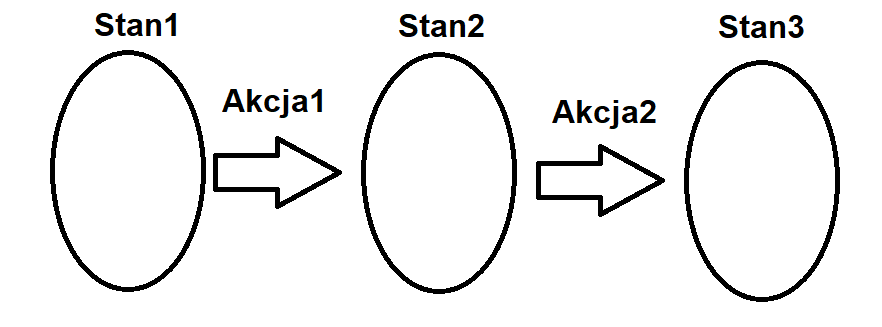
\includegraphics[scale=0.5]{PlanningGraph}
        \centering
        \caption{Najogólniejsza forma grafu planującego. Składa się on z węzłów, zwanych stanami oraz krawędzi zwanych akcjami. Docelowo poszczególne 
        stany oraz akcje są parami różne, jednak mogą zajść sytuacje, gdy powtórzenie któregoś z komponentów będzie wymagane do uzyskania odpowiedniego
        celu.}
        \label{PlanningGraph}
    \end{figure}
    Pierwotną ideę planu grafującego przedstawiono na obrazku \ref{PlanningGraph}. W trakcie dalszego omawiania metodologii GRAPHPLAN powyższa 
    rycina będzie pojawiała się ponownie z coraz to większym poziomiem szczegółowości.
    Ze względu na fakt, iż Graphplan opiera się na języku STRIPS musi mieć jasno zdefiniowane: stan początkowy, akcje oraz cel, który pragniemy uzyskać.
    Dzięki swojej strukturze Graphplan w swojej naturze podobny jest do programowania dynamicznego.

\section{Warunki początkowe}
    GRAPHPLAN, w odróżnieniu od człowieka, musi być w posiadaniu całej wiedzy o świecie, aby móc rozpocząć działanie. Przez całą wiedzę o świecie rozumie się
    posiadanie informacji na temat każdego obiektu oraz jego stanu. Przed dalszą częścią pracy należy dokonać pewnego wyróżnienia. Słowo \textbf{stan} pojawia się w dwóch znaczeniach:
    stan jako pojedyncza informacja o obiekcie w świecie (Przykład: klocek B na stole numer 3) oraz stan, jako zbiór wszystkich takich informacji w danym momencie czasu.
    Z tego względu wprowadzono nowe pojęcie- "Poziom stanów", które należy stosować jako oznaczenie wszystkich informacji o świecie w danym momencie.
    \begin{definition}
        \label{PoziomStanow}
            \textbf{Poziom stanów} - Zbiór informacji o stanach wszystkich obiektów w świecie w danej jednostce czasu \textit{t}
        \end{definition}
    Szczególnym poziomem stanów jest poziom oznaczany jako pierwszy i nazywany \textbf{Warunkami początkowymi}, którego poprawne zdefiniowane jest kluczowym aspektem w kontekscie
    uzyskania poprawnego wyniku przez algorytm.
    Analizując ponownie przykład \ref{Przyklad1} mylnym jest myśleć, iż jedyną informacją, jaką algorytm powinien posiadać o świecie jest pobyt klocka A na lewej platformie. Również
    istotną informacją jest brak klocka na platformie prawej, czyli informacja, ze jest on \textit{pusty}. Mimo poczucia nadmiarowości tej informacji, w dalszej części pracy wyjaśni
    się, dlaczego ta informacja jest niezbędna do uzyskania poprawnego wyniku.
    Przykład świata przedstawionego oraz skonstruowanego dla niego stanu początkowego:
    \begin{figure}[H]
        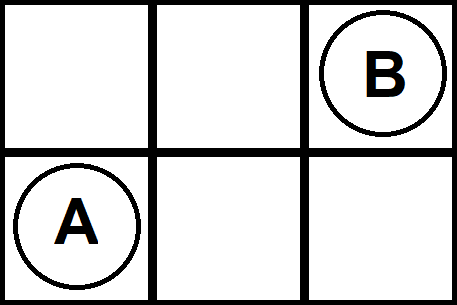
\includegraphics[scale=0.5]{PrzykladSP}
        \centering
        \caption{Przykładowy moment startowy przyszłego planu. Za pomocą okręgów oznaczono roboty, natomiast poprzez kwadraty oznaczone są kafelki- miejsca,
        po których mogą poruszać się roboty.}
        \label{PrzykladSP}
    \end{figure}
    Na powyższym przkładzie, zgodnie z powyższą ideą wyszczególniamy 6 stanów początkowych. Dodatkowo należy doprecyować pojęcie bycia robota na danym kafelku. Wykonano to 
    przy pomocy dwuargumentowej relacji \textit{na}, która jako pierwszy argument przyjmuje syngaturę robota, a na drugim- numer kafelka. Na potrzeby przykładu ustalono, iż 
    numerowanie odbywa się rzędami od prawej do lewej. Zgodnie z tymi ustaleniami pozycję robotów A i B możemy określić w następujący sposób: \textit{$na(A,4)$} oraz 
    \textit{$na(B,3)$}. Również pustość kafelków należy sformalizować wprowadzając relację jednoargumentową o nazwie \textit{pusty}, która przyjmuje jako argument numer
    pustego kafelka. Reasumując, zbiorem stanów początkowy dla analizowanego przykładu \ref{PrzykladSP} jest: 
    \begin{equation}
        \{pusty(1),pusty(2),na(B,3),na(A,4),pusty(5),pusty(6)\}
        \label{ZbiorPoczatkowy}
    \end{equation}
\section{Akcje}
    Posiadając dobrze określony stan początkowy następnym krokiem jest zabranie się za zdefiniowanie akcji. Zgodnie z \ref{Akcje} oraz wzmiance o akcjach w planerze STRIPS,
    akcja musi składać się z trzech komponentów:
    \begin{itemize}
        \item Czynności
        \item Warunków zajścia
        \item Efektów zajścia
    \end{itemize}
    Z tego powodu każdą z akcji będziemy traktować jako trójkę 
    \begin{equation}
        A=(C,W,E)
    \end{equation}
    gdzie każda z liter odpowiada pierwszej literze wyżej wymienionego pojęcia. 
    W skład efektów wchodzą dwa pojęcia wprost z terminologii STRIPS- dodające i usuwające. Dzięki takiemu podziałowi łatwiejszym będzie 
    zachowanie silnego podziału między przyczynami a efektami akcji. 
    Jedyną czynnością, którą należy brać pod uwagę w ramach \ref{PrzykladSP} jest czynność \textit{ruch}, którą definiujemy jako trzyargumentową relację:
    \begin{equation}
        ruch(R,S,D)
    \end{equation}
    , gdzie R odpowiada robotowi, który musi się przemieścić z kafelka oznaczonego literą S (kafelek startowy) na kafelek oznaczony
    literą D (kafelek docelowy).
    
    Drugą składową czynności są \textit{Warunki}. Warunki definiujemy jako następującą parę:
    \begin{equation}
        W=(D,U)
    \end{equation}
    gdzie D oznacza warunki dodające, a U- warunki usuwające.
    \begin{figure}[H]
        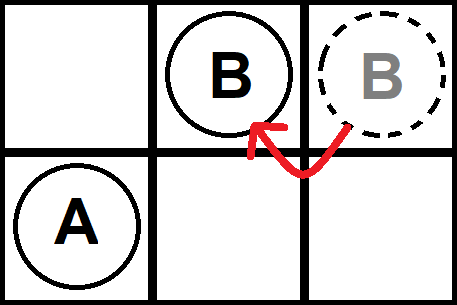
\includegraphics[scale=0.5]{PrzykladRuch}
        \centering
        \caption{Obrazowe przedstawienie ruchu robota B z kafelka 3 na kafelek 2}
        \label{PrzykladRuch}
    \end{figure}
    Niech rozpatrywaną akcją będzie przemieszczenie robota B z pozycji 3 na pozycję 2,
    przedstawiona na \ref{PrzykladRuch}. Biorąc pod uwagę, iż stanem początkowym jest \ref{ZbiorPoczatkowy} Warunkami zajścia zdarzenia
    będą: $na(R,S)$ oraz $pusty(D)$. Dla efektów natomiast sytuacja wygląda następująco: efektami dodającymi są $na(R,D)$ oraz $pusty(S)$, które informują o tym, iż klocek 
    zmienił swoje położenie, a efektami usuwającymi $~na(R,S)$ oraz $~pusty(D)$, które informują o tym, iż kafelek został zwolniony.

        Posiadająć następującą wiedzę poniżej zdefiniowano jedyną akcję znajdująca się w prezentowanym przykładzie:
    \begin{equation}
        A=(ruch(R,S,D),{na(R,S),pusty(D)},{na(R,D),pusty(S),~na(R,S),~pusty(D)})
    \end{equation}
    Podstawiając za $R=B$, $S=3$, a $D=2$ otrzymujemy następującą akcję: \\
        $A=(ruch(B,3,2),{na(B,3),pusty(2)},{na(B,2),pusty(3),~na(B,3),~pusty(2)})$
    
    Analogicznie można zdefiniować ruch na kafelek numer 6, oraz dwa ruchy dla robota o sygnaturze A.


    \subsection{Typy akcji}
        TO-DO: Akcje aktywne i pasywne

\section{Definiowanie świata}

\section{Warstwy grafu}

\section{Wzajemne wykluczanie}

\section{Równoległość}

\section{Wyszukiwanie planu}

\section{Prosty przykład}
